\documentclass[conference]{IEEEtran}
\usepackage{graphicx}
\usepackage{amsfonts}
\usepackage{amssymb}
%\usepackage[spanish]{babel}
\usepackage{verbatim}
\usepackage{amsbsy}
\usepackage{amsthm}
\usepackage{amsmath}
\usepackage{siunitx}
\usepackage{multicol}
\usepackage{xcolor}

\let\multicolmulticols\multicols
\let\endmulticolmulticols\endmulticols

\RenewDocumentEnvironment{multicols}{mO{}}
 {%
  \ifnum#1=1
    #2%
  \else % More than 1 column
    \multicolmulticols{#1}[#2]
  \fi
 }
 {%
  \ifnum#1=1
  \else % More than 1 column
    \endmulticolmulticols
  \fi
 }



\usepackage{algorithm}
\usepackage{algorithmic}
\usepackage[T1]{fontenc}		
\usepackage[utf8]{inputenc}
\usepackage{hyperref} 
\usepackage[super]{nth}
% correct bad hyphenation here
\usepackage{placeins} %para el FloatBarrier
\hyphenation{optical networks semiconductor IEEEtran}
%decimalpoint %decimales
%newtheorem{definition}{Definicion}[section]
%newtheorem{theorem}{Teorema}[section]
%newtheorem{lemma}{Lema}[section]

\theoremstyle{definition}
\newtheorem{definition}{Definition}[section]
\newcommand{\ts}{\textsuperscript}


\renewcommand{\abstractname}{\center\large Abstract \\}
\let\oldabstract\abstract
\renewcommand\abstract{%
  \begingroup
  \let\textit\relax
  \oldabstract
  \endgroup
  \bfseries
}

\usepackage{lipsum}
\usepackage{microtype}
\usepackage{lettrine}

\begin{document}

% paper title
\title{Automatic Tuning of Adaptive PID Controllers using an Artificial Neural Network}


% author names and affiliations
% use a multiple column layout for up to three different
% affiliations
\author{\IEEEauthorblockN{Soleiman N. Anwary, Charles W. Rigby}
\IEEEauthorblockA{Department of Process Systems Engineering, Imperial College London\\
\{sna314, cwr17\}@imperial.ac.uk}
}

% make the title area

% \pagestyle{plain}
% \maketitle
% \thispagestyle{plain}


\pagestyle{plain}
\twocolumn[
    \begin{@twocolumnfalse}
    \pagestyle{plain}
    \maketitle
    \thispagestyle{plain}
    \end{@twocolumnfalse}
    \begin{abstract}
    ~{Process control is an integral part of process systems anywhere in large scale production processes to applications in robotic devices. Specifically, we are interested in systematic control of bioprocesses due to their presence in sustainable generation of fossil-fuel alternatives. These systems are highly non-linear and display stochastic behaviour not easily modelled, creating a disparity in the plant-wide dynamics and model dynamics [Rio Del Chanona]. In this paper we investigate a black-box optimisation method through the use of a surrogate model to approximate the system dynamics and tune PID controller parameters through an gradient descent optimisation algorithm. We show that PID tuning parameters can be optimised for linear and non-linear systems without he intervention of manual methodologies such as Ziegler-Nichols or Cohen-Coon. We extended this model to multiple controllers whereby the surrogate model allowed communication between the the PID controller nodes in the artificial neural network. This multiple input and multiple output (MIMO) model is able to optimise PID controls for two different states of a system to various set point values for linear and non-linear systems so they reach stability given controllable system dynamics. \\

    \noindent \textit{Key words: Black-box, artificial neural network, process control, PID, tuning, control, Ziegler-Nichols, Cohen-Coon, surrogate model, deep reinforcement learning, Q-learning, MIMO, optimisation}}
    \end{abstract}
\bigskip]
\thispagestyle{plain}
% \begin{abstract}
% Process control is an integral part of process systems anywhere in large scale production processes to applications in robotic devices. Specifically, we are interested in systematic control of bioprocesses due to their presence in sustainable generation of fossil-fuel alternatives. These systems are highly non-linear and display stochastic behaviour not easily modelled, creating a disparity in the plant-wide dynamics and model dynamics [Rio Del Chanona]. In this paper we investigate a black-box optimisation method through the use of a surrogate model to approximate the system dynamics and tune PID controller parameters through an gradient descent optimisation algorithm. We show that PID tuning parameters can be optimised for linear and non-linear systems without he intervention of manual methodologies such as Ziegler-Nichols or Cohen-Coon. We extended this model to multiple controllers whereby the surrogate model allowed communication between the the PID controller nodes in the artificial neural network. This multiple input and multiple output (MIMO) model is able to optimise PID controls for two different states of a system to various set point values for linear and non-linear systems so they reach stability given controllable system dynamics. \\

% \noindent \textit{Key words: Black-box, artificial neural network, process control, PID, tuning, control, Ziegler-Nichols, Cohen-Coon, surrogate model, deep reinforcement learning, Q-learning, MIMO, optimisation}
% \end{abstract}

\IEEEpeerreviewmaketitle

\section{Introduction \& Motivation}
\lettrine{T}{he} topic of research considered in this paper covers a wide range of disciplines including process control, optimal control, black-box optimisation (BBO) and machine learning. Process feedback control dates back all the way to the third century BC. During this period Ktesibios of Alexandria employed a float valve to regulate the level in the water clocks used at that time [1]. Over the course of the subsequent centuries there was some development in process control, but it wasn’t until the industrial revolution that process control became widely utilised. The digital revolution coupled with the work of Russian American scientist Nicolas Minorsky on a formal control law (today known as PID control) [2] allowed for the development of modern computational control technologies which are used almost universally today in all process systems. Optimal control theory attempts to find a control law for a dynamical system that enables the system to perfectly respond to changes and disturbances. Ensuring optimal control is not straightforward and historically a large amount of effort has gone into designing approaches to solve this problem. Many of the systems that arise in chemical engineering problems are non-linear in nature [3]. This poses a problem when considering the control of such systems, as we may not have an easily tractable analytical expression that describes their responses to variations in the operating conditions. In this paper we aimed to address this problem by producing an algorithm which can find the optimal PID parameters to control a black-box system which is, by definition, a priori unknown. 

\noindent Black-Box optimisation methods are used in machine learning to find the minimum value of a real valued function that has no readily available analytical form. There are a wide variety of different BBO methods available including Genetic algorithms [4] and Particle Swarm algorithms [5]. The problem that we attempt to solve in the research paper can be described in its simplest form as follows: How can the optimum parameters to tune a PID controller for a black-box process system be found in an automated and systematic way? 

\noindent This is a vital problem to solve because an effectively tuned controller can provide a myriad of benefits in the operation of a process system. These benefits include but are not limited to ensuring product quality is maintained during operation by minimising the effects of process disturbances, establishing and maintaining process safety during operation and mitigating the time required, and the effects of, process start-up and shutdown. As the demands on the process industries grow over the coming years to serve an ever growing and increasingly affluent population, more energy and product wastage will occur in absolute terms. This highlights the importance of effective controller operation, and by extension controller tuning, as even small margins of unnecessary loss projected across time can lead to large unrealised profits for companies. Methods such as Ziegler-Nichols [6] and Cohen-Coon tuning [7] have been traditionally used to tune process controllers. Today these methods are  antiquated as they are time consuming and the controller parameters produced are generally not optimal. Currently in industry control engineers are increasingly turning to computational methods to optimise their control systems. Many of these methods rely on a knowledge of the physical system which for chemical engineering applications is generally unrealistic as the processes are highly complex in nature. Black-box optimisation methods can be exploited to provide a solution to this problem. In this research project we have considered a polynomial regression algorithm which approximates the true function by fitting a convex surrogate function. We can then apply a derivative based gradient descent to the surrogate function to determine the optimum point. To evaluate the effectiveness of this method requires us to consider the ease of implementation, the robustness of the method as well as how the dynamic system response is for the optimum tuning parameters.

The objectives of this research are primarily to have a robust algorithm which can be applied to determine the optimal control parameters for a wide range of systems. To do this we will consider a description of the proposed algorithm which provides the solution, an evaluation of the solution and a discussion of the algorithm performance and finally considerations about potential future improvements.
%--------------------METHODS------------------------
\section{Methods}
\noindent In this section of the report, we will set up and define explicitly, the exact form of the control system we used and how we set up the optimisation problem. We will then walk the reader through our algorithm which provides a solution to the problem for the single input single output case. Having arrived at a satisfactory solution for the preceding case we then consider the problem of multiple coupled controllers and how we can extend the functionality of the algorithm to tune both controllers simultaneously. 
\subsection{The Control System}
\noindent Figure 1. below is a representation of the feedback control loop. The value $x_{ref}$ is the set point desired for the process variable x. The difference between the set point and the process variable gives the error signal which is passed into the PID feedback controller which evaluates the error producing a controller response u. The controller response u then passes into the black-box system which determines a new value for the process variable x. The value of the error is then recalculated and the process repeats. If the PID controller is tuned correctly the error signal should decay over time and ideally reach a steady state value of zero. 

\begin{figure}[htbp]
\center{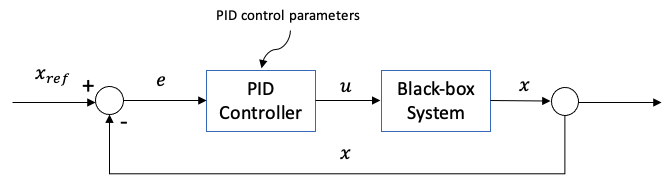
\includegraphics[width=0.48\textwidth]{9.png}}
\caption{test test test }
\label{kpki}
\end{figure}

\noindent The controller response u is determined using the following equation,
\begin{equation}
    u = \overbrace{k_p e(t)}^\text{P} + \overbrace{k_i \int_{0}^{\tau}e(\tau)d\tau}^\text{I} + \overbrace{k_d \frac{d}{dt}e(t)}^\text{D}.
\end{equation}

\noindent Where P, I and D correspond to the proportional, integral and derivative terms respectively. The coefficients $k_p$, $k_i$ and $k_d$ are the tuning parameters as these are the values which can be changed to tune the controller response u for a given error. The black-box system shown in Figure 1. is the process system which we are attempting to tune. In reality we would perform experiments on the system which we wish to tune, to collect data about the systems dynamic response for a given step change and tuning parameters, $k=[k_p,k_i,k_d]$. However, as this research is aimed at designing an algorithm to tune a wide variety of process systems, we instead simply define equations giving the change in the process variable for a given value of the process variable and a given controller response u. This allows us to test our algorithm on different systems, which is the main focus of this research. To ensure that the algorithm can tune a wide variety of systems we used equations with both linear and non-linear dynamics for testing,
\begin{equation}
    \dot{x} = 2x + u \textrm{ and } \dot{x} = x^2 + u.
\end{equation}

\subsection{The Optimisation Problem}
\noindent The decision variables for the optimisation problem are the values of, $k=[k_p,k_i,k_d]$ The different values for $\mathbf{k}$ give different dynamic responses for the control loop for a given black-box system. To determine which dynamic response is the best we define an objective function $\phi$. This function must minimise the total error over time and penalise large controller response values to ensure the response is smooth. The form of the objective function we arrive at is the following,
\begin{equation}
    \phi(x) = \sum_{i=0}^{N}(x_{ref} - x)^2_i + p\sum_{i=0}^{N}u_i^2
\end{equation}

\noindent Where the first term is the square error summed over N discrete time steps and the second term in the equation is the square of the controller response multiplied by a penalty coefficient $p$. The second term is not essential for the minimisation, but it will help add greater curvature to the approximation of the function $\phi$ which becomes important for visualisation later. The greater the value of the penalty coefficient $p$ the greater the added curvature. For our purposes we determined that $p=2$ was sufficient.

\subsection{The Algorithm}
\noindent In this section we describe the steps the algorithm takes to find the value for the optimal control parameters $\mathbf{k}^*$. For a depiction of the algorithm in schematic form please see the Appendix A for the algorithm flowchart. Please also note that information regarding the implementation of the algorithm in Python is given in the Appendix.

\noindent The first step the algorithm takes is to define upper and lower bounds for the values of the control parameter $\mathbf{k}$. The lower bound on the parameter values is zero due to the way the control response function is defined. This means that if we define a 3D space for the possible values of $k_p, k_i$ and $k_d$, with each dimension corresponding to a control parameter, that the space is restricted to the positive octant of the 3D region. The upper bound on the control parameters is defined such that an initial mesh of values can be produced in the 3D space. Note that the upper and lower bound values will be redefined as the algorithm iterates so it is not imperative that the upper bound constrains the problem such that the optimum value is in the initial region. This will become clear when we discuss the bound redefinitions later. The initial upper bound value we chose for all control parameters was $k_{ub}=5$.

\noindent Once the bounds have been established for k the algorithm creates a low-resolution mesh of points within the 3D space defined by the bounds. Each point or node in the space defines a unique combination of $k_p, k_i$ and $k_d$. The algorithm uses the number of points on each axis between the bounds as 10. The algorithm then performs a dynamic simulation for each node using the defined control system. For each simulation the value of the objective function is evaluated. Therefore, for every node in the 3D space we have a value for the objective function $\phi$.

\noindent To perform a dynamical simulation the algorithm defines a total time for the dynamical simulation T and a discrete number of steps N. The simulation then proceeds by determining the initial value for the error $e_0$ and storing it. The error is then passed into the controller which evaluates the controller response function as described earlier for $t=0$ giving a value $u_0$ which is then stored. The black box function is then used to evaluate a new value of x at time Dt, where $Dt = T/N$. This new value of x is used to calculate a new value for the error, which is again stored and the process loops until time equals T. The store of error and controller response values at the end of the simulation is used to calculate the value of $\phi$ for that simulation.

\noindent As discrete time is used for the simulations a discrete version of the controller response function is used which is defined below,
\begin{equation}
    u_n = k_p e_n + k_i \sum_{i=0}^{N}e_i + k_d \frac{e_n - e_{n-1}}{Dt}.
\end{equation}

\noindent We can now use a regression technique to fit an approximate or surrogate function to the values of $\phi$ in the space. The method we use is the sequential least squares programming method from minimize in the scipy.optimize package. The approximate function we fit, $\phi_{approx}$, is a convex quadratic function of the following form,
\begin{equation}
    \phi_{approx}(x) = \mathbf{k} \cdot Q \cdot \mathbf{k}^T + \mathbf{c} \cdot \mathbf{k}^T,
\end{equation}
Where,
\begin{equation}
    \mathbf{c} = [c_1, c_2, c_3] \textrm{ and } Q = \begin{bmatrix}
                                                    Q_1 & 0 & 0 \\
                                                    0 & Q_2 & 0 \\
                                                    0 & 0 & Q_3 \\
                                                    \end{bmatrix}.
\end{equation}

\noindent The parameters that we use to fit $\phi$ to $\phi_{approx}$ are the $\mathbf{c}$ and $Q$ values. The reason that the off-diagonal terms in $Q$ are zero is such that the approximate function retains its convexity and remains easily solvable to its global minimum. 

\noindent Once we have an analytical expression for $\phi_{approx}$ we can then minimise this function again using minimize from scipy.optimize to get the optimum values for $\mathbf{k}$  for the first iteration. With the optimum $k_1^*$ values we can reset and tighten the bounds around $\mathbf{k}$ using the following equations,
\begin{equation}
    \textrm{Do this later on - Sol }
\end{equation} 

\noindent With the new values for the bounds, we can define a tighter mesh in the positive octant with the same number of nodes as before. We then iterate the entire process until the optimum $\mathbf{k}^*$ values converge. 

\noindent The reason we set up the algorithm to iterate in this way is due to the fact that each dynamic simulation for each unique value of $\mathbf{k}$ is computationally demanding and therefore, we want to minimise the required number of simulations to get to the optimum $\mathbf{k}^*$. In order to minimise the number of dynamic simulations we have the number of points on each axis, as specified earlier, as 10. This gives enough information to fit the approximate function to $\phi$ with a reasonable degree of accuracy. However, the accuracy of the fit is not high enough for us to conclude that the optimum $\mathbf{k}^* \approx \mathbf{k}_{approx}^*$ on the first iteration. Therefore, we must iteratively reduce the bounds, for the same number of points on each axis. This ensures as the number of iterations increases the resolution also increases eventually allowing us to approximate $\mathbf{k}^* \approx k_{approx}^*$ for a high enough number of iterations.

\subsection{Coupled Controllers with Multiple Inputs and Multiple Outputs}
\begin{figure}
    \centering
    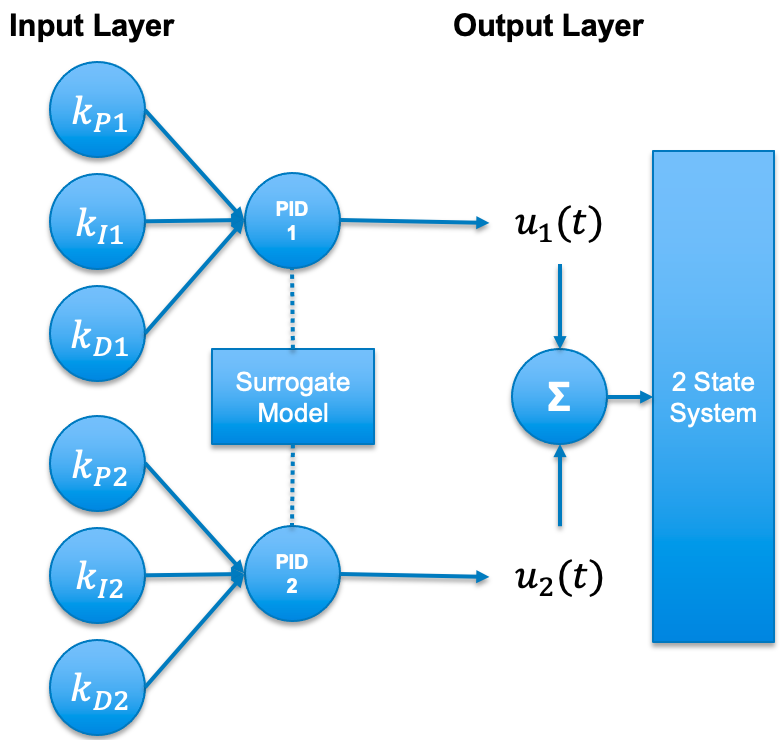
\includegraphics[width=0.45\textwidth]{NN.png}
    \caption{Artificial Neural Network}
    \label{fig:my_label}
\end{figure}
\noindent In a real process system, there will likely be cases where two or more controllers will be coupled. This means that it may be that the controllers act antagonistically and when the tuning parameters for one controller are optimised the other controllers may not be able to operate optimally. This is the problem of multiple input multiple output (MIMO) controller optimisation.
%--------------------- MATHEMATICAL AND COMPUTATIONAL ASPECTS ------------------
\section{Mathematical \& Computational Aspects}
\noindent We are addressing the problem of tuning parameter optimisation using a surrogate machine learning model. We are using a quadratic approximation to the actual dynamics of the system. For this problem to be soluble the surrogate model has to be convex and all the constraints must also be convex such that the problem overall is convex. \\
\theoremstyle{definition}
\begin{definition}
\textit{A function f}: $\mathbb{R}^n \rightarrow \mathbb{R}$ \textit{is convex if and only if its domain is a convex set $\forall$ $x, y$ and all $\lambda \in [0,1]$. } 
\end{definition}
\noindent A multivariate quadratic function such as the surrogate model
\begin{equation}
    f(x) = \mathbf{k}Q\mathbf{k}^T + \mathbf{c}\mathbf{k}^T,
\end{equation}
\begin{equation}
    \mathbf{c} = [c_1, c_2, c_3] \textrm{ and } Q = \begin{bmatrix}
                                                    Q_1 & 0 & 0 \\
                                                    0 & Q_2 & 0 \\
                                                    0 & 0 & Q_3 \\
                                                    \end{bmatrix}
\end{equation}
is convex if and only if $Q \succcurlyeq 0$. This is important because it means that the quadratic coefficients of the surrogate model have to be constrained to non-negative values. So by defining Q to be a symmetric matrix and the constraining the quadratic term coefficients to be non-negative we ensure all eigenvalues of the matrix are positive and as such the matrix $Q$ is positive semi-definite which keeps the optimisation problem convex. Most importantly, a convex system means any local minimum found is also a global minimum. 


%--------------------------RESULTS AND DISCUSSION------------------------------------
\section{Results \& Discussion}
\subsection{Optimisation of a 2D Control System}
\begin{figure*}[h]
    \setlength{\abovecaptionskip}{0pt}
    \center{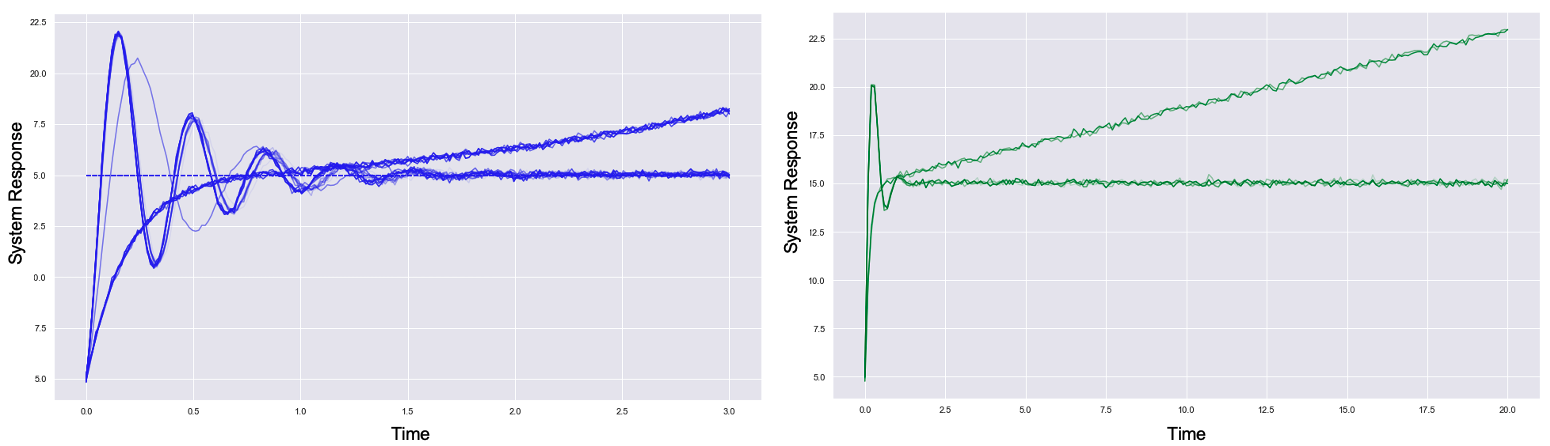
\includegraphics[width=\textwidth]{1.png}}
    \caption{The system responses shown are for the 2D case where we optimised only the tuning parameters $k_p$ and $k_i$. The above two graphs show the system response history for each iteration that the algorithm runs for a linear (blue) and a non-linear (green) system, respectively. The system was run 40 iterations and samples at every \nth{10} iteration. We observe system stability being reached for each experiment.}
    \label{kpki}
\end{figure*}

\begin{figure*}[h]
    \center{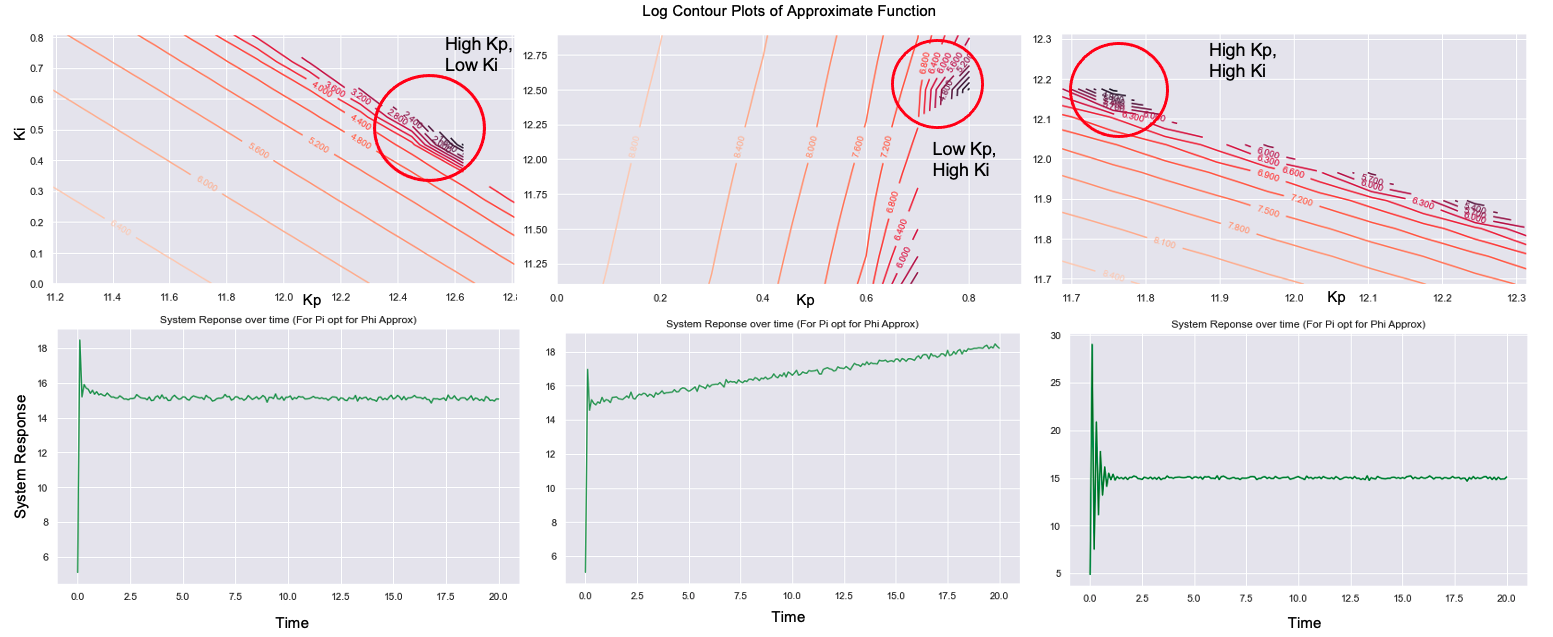
\includegraphics[width=\textwidth]{2.png}}
    \caption{The above figure shows log contour plots of the approximate function $\phi_{approx}$ for 3 different scenarios from left to right: a) system convergence, b) system divergence and c) oscillatory system response with convergence. Regions where the surrogate function estimates a minimum we see greater curvature and these regions are highlighted with a red circle and a corresponding annotation about the value of the tuning parameters. The experiments were conducted over linear system dynamics.}
    \label{kpki_contour}
\end{figure*}

\begin{figure*}[h]
    \center{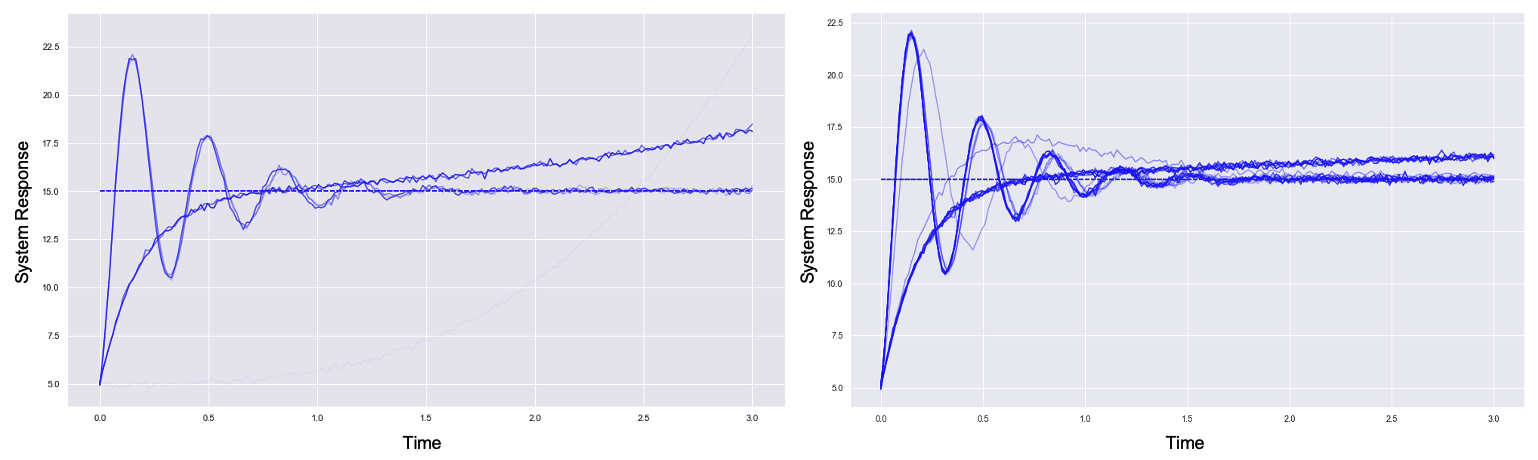
\includegraphics[width=\textwidth]{3.png}}
    \caption{The system responses shown are for the 3D case where we optimised the tuning parameters $k_p$, $k_i$ and $k_d$. The above two graphs show the system response history for each iteration that the algorithm runs for a linear (blue) and a non-linear (green) system, respectively. The system was run 40 iterations and samples at every \nth{10} iteration. We observe system stability being reached for each experiment.}
    \label{kpkikd}
\end{figure*}

\begin{figure*}[h]
    \center{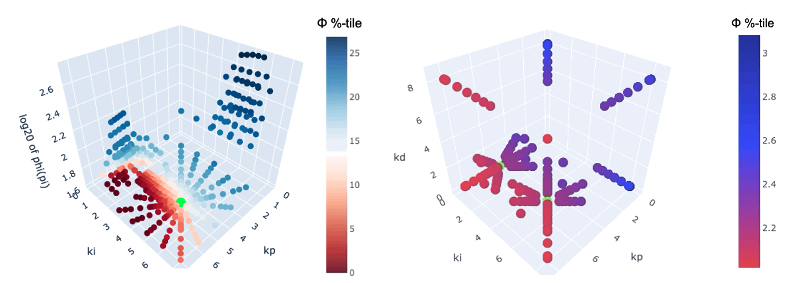
\includegraphics[width=\textwidth]{8.png}}
    \caption{\lipsum[2]}
    \label{3D_plots}
\end{figure*}

\begin{figure*}[h]
    \center{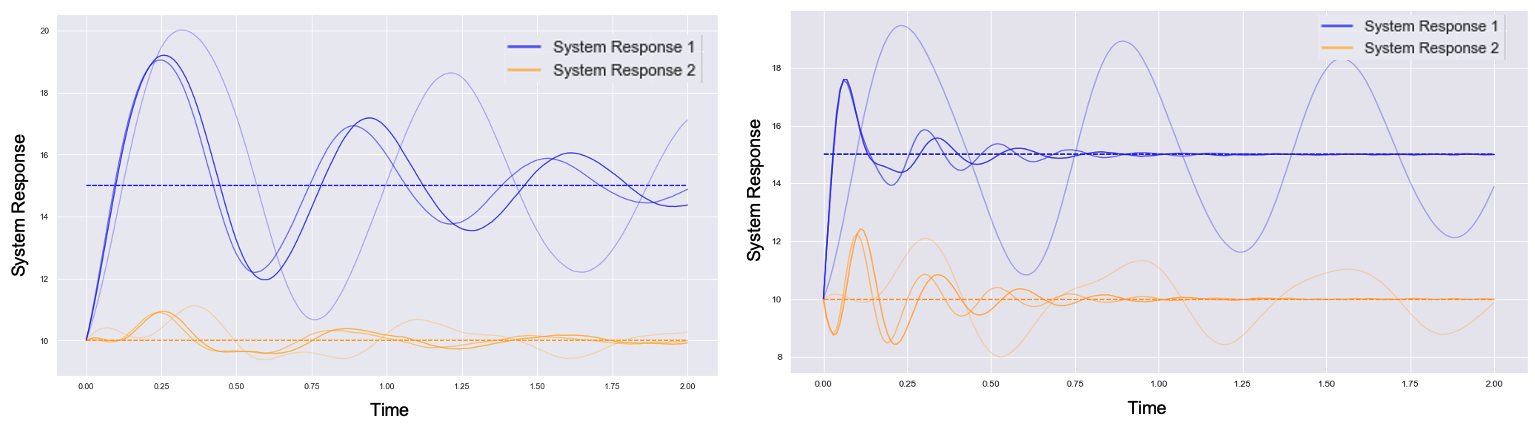
\includegraphics[width=\textwidth]{5.png}}
    \caption{\lipsum[2]}
    \label{mimo_smooth}
\end{figure*}

\begin{figure*}[h]
    \center{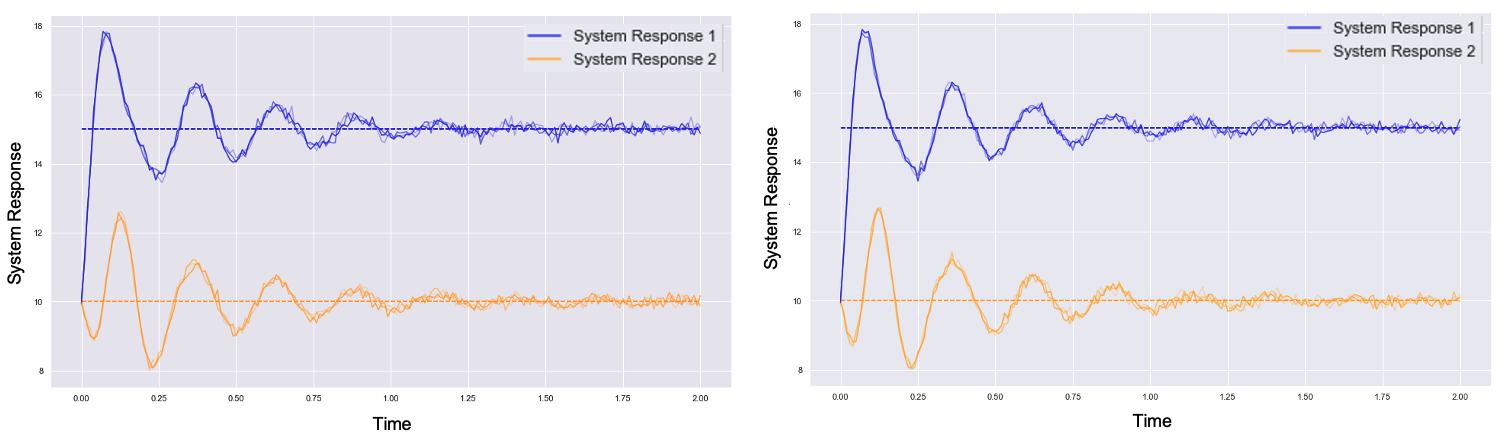
\includegraphics[width=\textwidth]{6.png}}
    \caption{\lipsum[2]}
    \label{mimo_rough}
\end{figure*}

When optimising a control system we first had to segment the problem. The majority of dynamic systems are controllable using a P and I control system [Reference]. With this in mind, we pose the hypothesis: the algorithm should come to the conclusion that the majority of systems tested are PI-controllable. Indeed what we observed was that both linear and non-linear system dynamics were controllable and converged onto a set point; a number of set points were used to test model robustness and in each case the model presented a converging system response. We can see Figure X shows system responses for the optimal set of tuning parameters, $k_p$ and $k_i$  as determined by the surrogate model optimisation. Several iterations of the model were plotted on the same axis to show how the algorithm parses through the mesh of tuning parameters generated. The darker lines represent later iterations and the latest updates to the optimal response. The following were used as benchmark dynamic systems to test the model performance:
\begin{equation}
\dot{x} = 2x +u \quad \textrm{and} \quad \dot{x} = x^2 + u
\end{equation}
It is important to note the algorithm is designed to work on unknown system dynamics; the outputs of the system would be gathered and fed into the algorithm as an input. This would be used by the model to fit an approximate surrogate function and find the optimal tuning parameters.\\
The cost function $\phi$ is evaluated at each iteration and plotted over the parameter vector space to visualise the surface. We do this in a 3-dimensional plot of $k_p$ against $k_i$ and $\phi$. The value of $\phi$ is broken into percentiles and categorised in the plot using a continuous colour scale. It can be seen the cost function $\phi$ predicts the optimal value of $\boldsymbol \pi$ to be in the region with low $k_i$ and high $k_p$ values. The sample space in the parameter mesh is cubic and this is seen in the plot. The surrogate function $\phi_{approx}$ predicts the optimal $\boldsymbol \pi$ to be at $(5,5)$. This is not completely consistent with what the cost function predicts. This may be because the surrogate model is sampled far more around that point and as such a greater weight is given for that set of values as the optimum $\boldsymbol \pi$. A higher density plot of phi was generated to test this and indeed the optimum predicted by the surrogate function moved closer to the darker red region where $\phi$ is minimised [figure reference].
Furthermore, while low values of the integral term are preferred - which controls how smooth the system response is - a zero value for $k_i$ is not. Without any integral action the system response starts oscillating and often results in a steady state error. We therefore suggest that a PI-control system is sufficient for most linear and non-linear systems with first order dynamics. 

\subsection{$\phi_{approx}$ vs. $\phi$ fit }
We investigated the agreement between the surrogate function $\phi_{approx}$ and the cost function $\phi$ in Figure X. Comparing the contours to the 3-dimensional scatter plot for $\phi$ in Figure X shows us that there is a large flat region before the surface shows curvature. This is seen in the contour plots. More specifically, there are three cases which were isolated for analysis: a) system convergence, b) divergence and c) fast oscillatory system response. In case a) we can see that the contour starts curving to a minimum which is in a region with a high $k_p$ and low (and non-zero) $k_i$ value. This is consistent with the predictions from the cost function alone. We can see the system reaches a steady state set point value preset at 15 for this experiment. Case b) presents a case where the contour is approaching a point which is in a region with low $k_p$ and high $k_i$. It is clear that when the proportional gain is not large enough the system is not only slow to respond (large rise time) it is also unable to reach a steady state value and therefore stability. The final case is the last iteration of the experiment and shows that a possible system response is one with both $k_p$ and $k_i$ at the boundary of the active constraints set; here we observe large initial overshoot and initial oscillations which are brought about by the larger integral term. 

\subsection{Optimisation of a 3D Control System}
We extended the PI-control parameter optimisation to the 3D case by also considering a derivative term, $k_d$. Figure X shows various system dynamics and how the model handled the optimisation to achieve a steady state system response for both linear and non-linear system dynamics. Once again we used several set point values to test the model and system response convergence. All tests showed the model successfully corrected for the step input error and brought the system back to the set point. There are several values of $\boldsymbol \pi$ which led to a sub-optimal response where the system slowly diverged from the set point. However, the last batch of iterations show that the most intensely coloured blue lines belong to the group of $\boldsymbol \pi$ solutions which yield a steady state system response. It was also important to understand how the cost function behaved across the parameter space. Figure X shows a 4-dimensional plot of the parameters $k_p, k_i, k_d$ and the value of $\phi$ normalised as a percentile as the 4\ts{th} dimension which is shown as colour in this instance. We can see that once again a high value of $k_p$ and low but non-zero values of $k_i$ are preferred by the model for linear and simple non-linear dynamics. The parameter $k_d$ is often very close to or in fact \textit{zero}. This reinforces the model's PI-control preference; it suggests that a proportional gain and a small integral error correction mode are sufficient to control most systems effectively. Furthermore, the surrogate approximate function $\phi_{approx}$ attempts to find optimal values for $\boldsymbol \pi$ in the region where the derivative term is zero, and the proportional and integral terms are equal because the model samples heavily in that region. This suggests that there is a compromise that has to be achieved for the surrogate model. It can either try to approximate the system dynamics in small local spaces which would improve the fit between $\phi$ and $\phi_{approx}$ or it can approximate the dynamics globally which means that $\phi_{approx}$ cannot be accurate across the whole domain. The model is designed to be memoryless - upon each iteration the model does not retain any state space variables describing the system or the tuning parameters which were used in the previous iteration prior to bound reduction. As a result, the approximate surrogate function inherently will not be able to approximate the system dynamics equally well over the entire space. 

\subsection{Multiple Input Multiple Output Control System (MIMO)}
When designing the control algorithm it was important to consider use-case scenarios for its application. One such use-case is in biochemical processes. Biochemical processes utilise biological microorganisms to produce chemical derivatives and high-value products otherwise too complicated to obtain through physical chemical modes. However, the complex interactions between the substrates in metabolic pathways and the culture fluid dynamics makes bioprocess control particularly challenging to control [Reference Rio del Chanona, Reinforcement learning for batch bioprocess optimization]. System-wide or plant model dynamics cannot meaningfully be obtained for such processes and as such they must be treated as black-box models. Often there are multiple controlled variables such as pH, feed stock concentration, product concentration, temperature, pressure and flow rate; many of these parameters are dependant on each other and as such a control system which can allow communication between multiple controllers which correct related system states is important. \\
As such we have developed an artificial neural network (ANN) for multiple controllers which are linked to each other by a surrogate model function - in this case $\phi_{approx}$. This surrogate model will allow the controllers to communicate and compromise on the optimisation of the tuning parameters to reach system stability. The tuning parameters make up the weights of each distinct error term in the input layer, allowing the controllers to generate control functions as the output. With that in mind we tested the extended model on two controllers and applied it to both linear and non-linear systems,
\begin{align}
    \dot{x_1} &= 2x_1 + x_2 +2u_1 - u_2 \\
    \dot{x_2} &= x_1 + 2x_2 - 2u_1 + 2u_2.
\end{align}

\noindent Figure X shows both system dynamics were brought to stability using the optimised tuning parameters. The history of how the model reached the optimal system response is shown. Upon addition of disturbance to the environment and noise to the controllers we optimised the tuning parameters and achieved stability for both the linear and non-linear system as is shown in part b) of Figure X. This model can be tested for $n$ number of controllers and the optimisation algorithm will coordinate the controllers since the optimiser adjusts the weights of the proportional, integral and derivative term for all controllers simultaneously. This makes the surrogate function a communication pathway to reach a globally optimal solution while exerting control on all system variables.


%----------------------------LIMITATIONS AND COMPLEXITIES------------------------
\subsection{Limitations \& Complexities}
\subsubsection{Stochasticity}
\noindent When developing this blackbox optimisation model we added disturbance and noise to the system environment and control system itself, respectively. This was done to test the robustness of the algorithm to sudden and small changes and simulate a stochastic version of the model. A non-robust controller would explode the derivative term in response to the uneven characteristics of the system response if the tuning parameters are not optimised correctly. Interestingly, we saw that the model was able to bring linear and non-linear systems to stability but at the costs of removing the derivative term entirely. This may be because the derivative term, while reducing the initial overshoot of the system, would become too sensitive to disturbance and noise from the environment and controller, respectively. We used a frozen Gaussian probability density function (one where the mean and standard deviation is fixed for each random variable generated) to add the complexity of disturbance and noise as given by,
\begin{equation}
    p(x) = \frac{1}{\sqrt{2\pi \sigma^2}} \exp{\left\{-\frac{ (x-\mu)^2}{2\sigma^2} \right\}}
\end{equation}
\vspace{1mm}
\noindent Where $\mu$ is the mean and $\sigma$ is the standard deviation. A mean of $\mu=0$ and standard deviation of $\sigma=0.2$ were used. 

\subsubsection{Hyperparameter Optimisation}
There were several hyperparameters which we did not yet optimise for in this model. These include the number of iterations the neural network needs to run to each an optimum value, the size of the network itself, and the activation function for the optimisation. Blackbox optimisation problems rapidly become computationally expensive. This is apparent when looking at the architecture of the ANN for the MIMO system. Each controller commands a set of six coefficients and three tuning parameters in the surrogate function and with a sample space as small as two samples per tuning parameter the space grows exponentially by $(2n)^i$ where $n$ is the number of nodes and $i$ represents the dimensionality of the vector space, 3, in this case. As such we only tested the MIMO system using two controllers as we were running all simulations on a 2014 \SI{2.2}{GHz} Quad-Core i7 processor chip. 

Currently, we are using a linear activation function in the PID controller i.e. the $u$ function. This means that the current neural network cannot stack several layers because irrespective of the number of layers in the neural network the activation of the output layer is simply going to be a linear combination of the input of the first layer. This can be overcome by replacing the linear activation function with a non-linear function such as a Sigmoid function or a hyperbolic tangent function like below, 
\begin{align}
    s(x) &= \frac{1}{1 + e^{-x}} \\
    f(x) &= \tanh(x) = \frac{1}{1+e^{-2x}}.
\end{align}
%-------------------OUTLOOK AND FURTHER WORK------------------------------  
\section{Outlook \& Further Work}
\subsubsection{Non-linear Activation Function}
As previously alluded to, it would be important to ascertain the model's behaviour with a non-linear activation function; this would be in pursuit of creating a better fit between the system dynamics and the approximate surrogate function globally across the entire sample domain.
\subsubsection{Step Change Input}
It would be most curious to train the neural net on a set of different disturbances and step input changes so that the model is able to handle large changes in the environment more effectively. This would involve prediction of optimal tuning parameters for specific step changes. 
\subsubsection{Gaussian Processes}
In this paper we have explored the use of a convex quadratic function to approximate the system dynamics. However, studies have shown that using Gaussian processes in place of a quadratic function can yield better results for global optimisation problems [Osborne, M. A., Garnett, R., \& Roberts, S. J. (2009). Gaussian processes for global optimisation]. Gaussien Processes are a generalisation of the Gaussian probability distribution. While probability distributions can describe random variables, Gaussian processes (which are stochastic bu definition) describe properties of functions over a finite space [Rasmussen Book]. One of the reasons why Gaussian processes may be a better fit for this than a quadratic function might be because the presence of significant stochastic uncertainties in a system environment can lead to closed-loop performance and uncontrollability issues. GPs can be used to formulate nonlinear constraints for non-linear systems and thus improve control performance [Bradford, 2018  Stochastic Nonlinear Model Predictive Control Using Gaussian Processes]
\subsubsection{Reinforcement Learning - Q-learning}
\begin{figure}
    \center{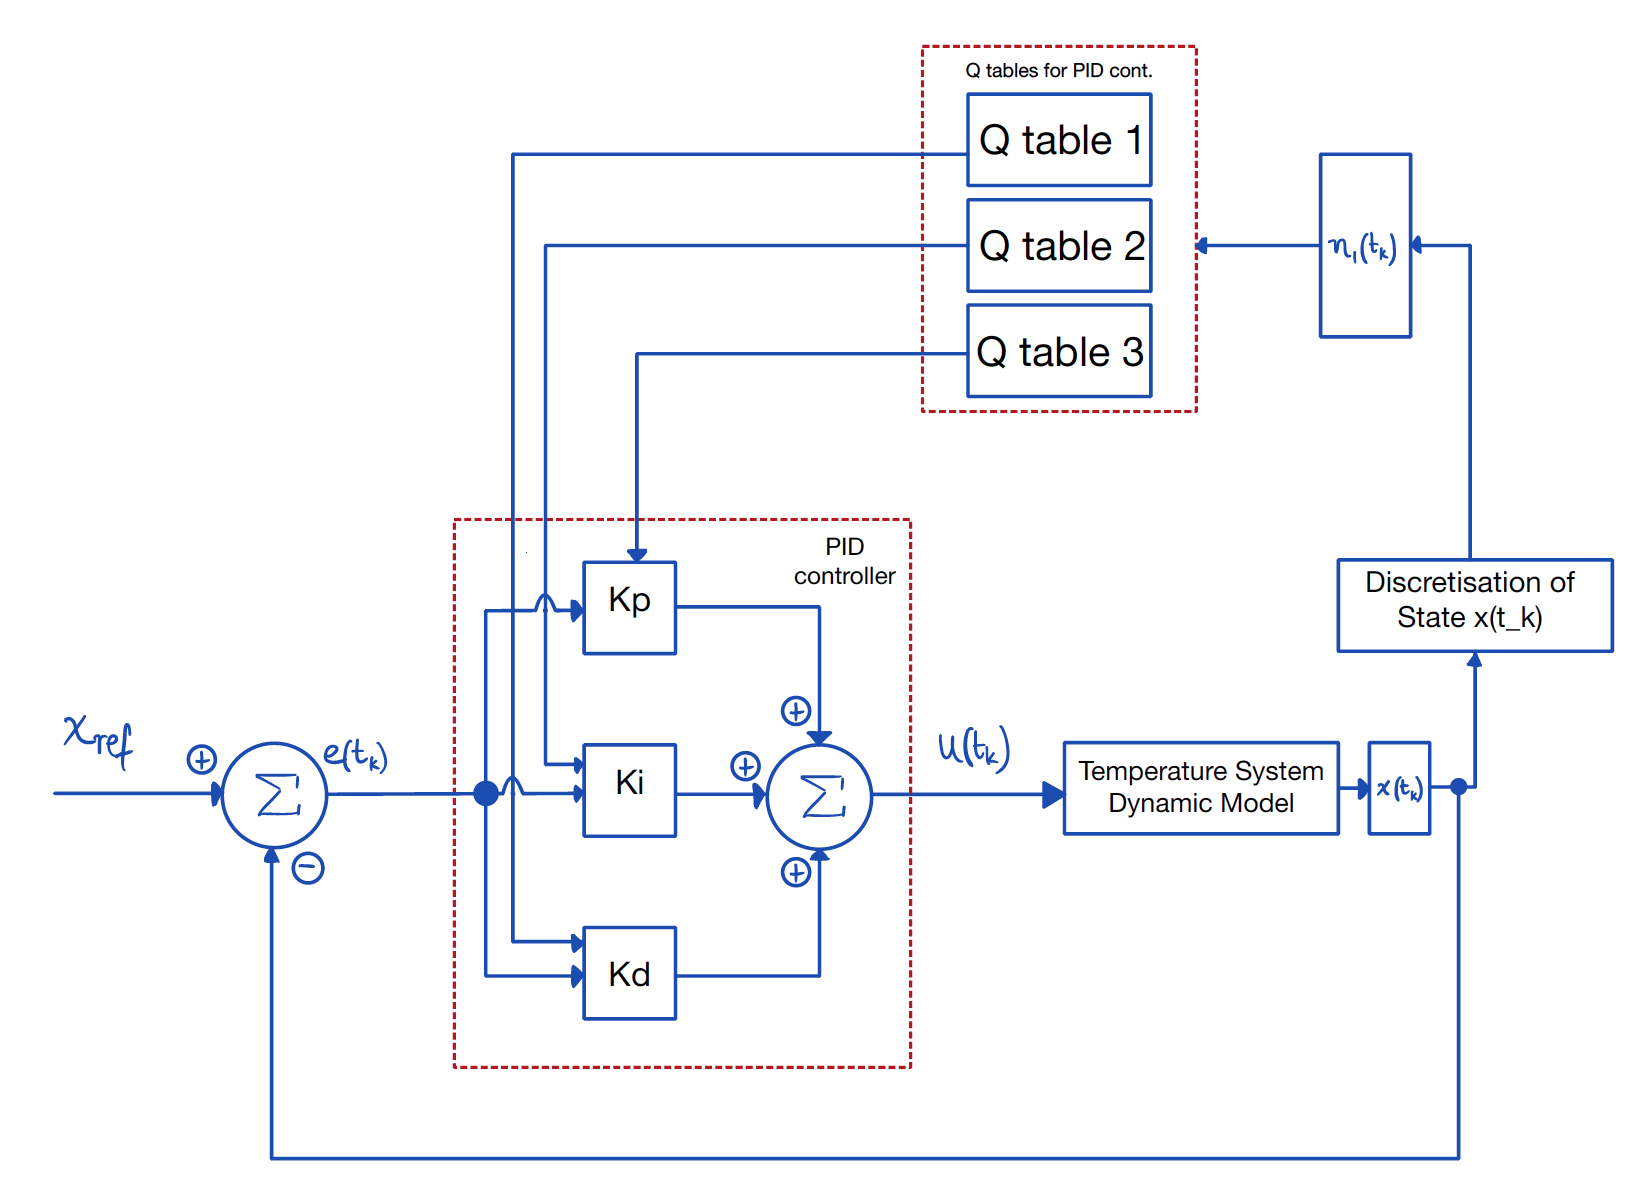
\includegraphics[width=0.499\textwidth]{7.png}}
    \caption{Adaptive PID controller Q-learning architecture proposed for future work on this project}
    \label{q-learning}
\end{figure}
Reinforcement learning (RL) is a particular branch of dynamic programming which has previously been applied to control systems by completely replacing PID controllers [6]. Ramanathan et. al. used Q-learning to control the fluid level in a non-linear conical tank and observed good performance [7]. A problem with replacing PID controllers with RL algorithms is that these algorithms heavily rely on the state space representation of the problem; that is, the architecture of the input, output and the system's dynamical equations. 
Research has emerged where RL/PID control hybrid algorithms have been proposed using techniques such as Discrete Action Reinforcement Learning Automata [13] to tune PID control parameters with a higher learning rate than RL algorithms alone. Actor-critic methods have also been proposed to optimally tune controllers [18] for wind turbines: the actor maps states to the PID tuning parameters and the critic evaluates the output of the actor[THE paper, and 14]. Quality learning (Q-learning) is being used in tuning single PID controllers [19] and recently experiments have shown they can be applied to multiple controllers [THE Paper]. Q-learning incorporates the importance of an agent's ability to both explore and exploit the environment's resources. Q-learning leverages the dynamic nature of policy rewards such that the process of controlling a system becomes dynamic; instead of having a static set of gains for a PID control systems in an attempt to control a dynamic environment, Q-learning changes the weights of tuning parameters dynamically to suit the particular disturbances sensed from the environment. This means a PID controller can directly control a system which is simple while allowing the Q-learning algorithm to dynamically adjust the control function to adapt to more complex and non-linear systems and situations. With this in mind, we created a simplistic Q-learning architecture schema for the control of a single PID controller as seen in Figure [X]. This kind of approach can be taken for further investigation of Q-learning RL/PID hybrid control algorithms for systems such as bioprocess systems.

%---------------------CONCLUSION-----------------------------

\section{Conclusion}
\noindent Having performed all of the simulations we are able to draw some conclusions about both the algorithm and the general field. We hypothesised that as PI control was generally sufficient for most cases in the process industry it would likely be sufficient to control many of the black-box systems trialled on the algorithm. We determined that this was indeed the case as when the algorithm was trialled for simple PI control it returned $k_p$ and $k_i$ values which allowed the system to respond well to the given step changes. 

To be successful it was also important for the algorithm to be able to determine optimum tuning parameters for a wide range of different system types. As seen in the results and discussion the algorithm was able to predict the optimum tuning parameters for both linear and non-linear black-box systems. This reflects positively on the algorithms robustness. However, to be able to formally define our algorithm as robust it would be necessary for us the test the algorithm on a very wide range of system dynamics. This unfortunately was not feasible for us to achieve as our time to produce this research was very limited, but it is something that we would wish to consider in future work in this area. For the algorithm to be of any practical use it would have to be able to tune a number of linked controllers. In our testing the algorithm was able to tune two linked controllers. This functionality can be extended to any number of linked controllers. The constraining factor in our testing was the dimensionality of the problem with the increase in the number of controllers. The increase in the dimensionality of the problem simply made testing on any more than two linked controllers infeasible due to the increase in computation time. With access to HPC computers the algorithm would be able to effectively tune the parameters for any number of controllers. An interesting area for further research would be to look into methods of dimensionality reduction. 

Perhaps the most important conclusion of this research is that the algorithm was successful in its primary objective which was to provide an automated and systematic way of tuning the control parameters for a black-box system. This is a particularly striking result as it demonstrates that with access to data about system responses and with no further knowledge of the actual system dynamics, it is possible to effectively find its optimum tuning parameters. This removes the need for any manual intervention using tuning methods, which in turn means that system operators need not be trained extensively in the methods by which control systems are tuned. It also means that any inefficiencies that arise from these tuning methods can be disregarded which would be beneficial in the operation of process systems due to more capable responses to disturbances and step changes that would be produced by the PID controllers. 

%--------------------ACKNOWLEDGEMENTS------------------------
\section{Acknowledgements}
\noindent We would like to extend the warmest thanks to our research supervisors Professor Antonio Del Rio Chanona, Dr. Panos Petsagkourakis, and Ilya Orson Sandoval for their continued technical support and mentorship throughout the project. 
































%\begin{displaymath}
%[y]^- = -yI(-y) \textrm{, con } I(-y)=\left\lbrace 
%	\begin{array}{cc}
%	1	&	\textrm{ si } y < 0	\\
%	0	&	\textrm{ otro caso}
%	\end{array} \right.
%\end{displaymath}


%\begin{algorithm}
%{\footnotesize
%\caption{Quadratic Penalty}
%\label{algQuadPen}
%\begin{algorithmic}[1]
%\STATE Given $(\mu_0 > 0$, tolerance $\tau_0$, starting point $x_0^s$
%\FOR{$k=0,1,2\ldots$}
%\STATE Find an approximate minimizer $x_k$ of $Q(\cdot;\mu_k)$, starting at $x_k^s$, and terminating when $||\nabla Q(x;\mu_k)||\leq \tau_k$
%\IF{final convergence test satisfied}
%\STATE \textbf{STOP} with approximate solution $x_k$
%\ENDIF
%\STATE Choose new penalty parameter $\mu_{k+1} \in (0,\mu_k)$
%\STATE Choose new starting point $x_{k+1}^s$
%\ENDFOR
%\end{algorithmic}}
%\end{algorithm}



%{\footnotesize
%\begin{eqnarray}\label{eqgrad}
%\nabla_x \mathcal{L}_A(x_k,\lambda^k;\mu_k) & = & \nabla f(x_k) - \sum_{i\in \mathcal{I}|c_i(x)\leq\mu\lambda_i^k} \left(\lambda_i^k - \frac{c_i(x_k)}{\mu_k} \right) \nabla c_i(x_k)	\nonumber \\
%\end{eqnarray}
%}


%\begin{table}[htbp]
%\begin{center}
%\begin{tabular}{|c|c|c|c|}
%\hline
%			& Penalizaci\'on Cuadr\'atica		&	Barrera Logar\'itmica	&	Lagrangiano Aumentado	\\
%\hline
%$f(x^{*})$	& 0.1643	&	0.1774	&	0.1642	\\
%\hline
%\end{tabular}
%\caption{Resultados para cada m\'etodo en el problema a optimizar.}
%\label{tresults1}
%\end{center}
%\end{table}
\begin{thebibliography}{1}
\bibitem{Arpack}
Richard B Lehoucq, Danny C Sorensen, and Chao Yang, \textit{ARPACK users' guide: solution of large-scale eigenvalue problems with implicitly restarted Arnoldi methods}, volume 6. Siam, 1998.

\bibitem{Elixir}
Developmented by José Valim for Plataformatec, \emph{Elixir} , \url{https://elixir-lang.org/}
\bibitem{Facebook}
Facebook Inc, \emph{Facebook}, 2018 and \url{https://www.facebook.com/}

\bibitem{github}
GitHub ,Inc., \emph{GitHub}, 2018 and \url{https://github.com/}

\bibitem{MatrixC}
G.H. Golub and C.F. Van Loan, \emph{Matrix Computations}, John
Hopkins Press, 1989.

\bibitem{MatrixSpark}
Bosagh Zadeh, Reza and Meng, Xiangrui and Ulanov, Alexander and Yavuz, Burak and Pu, Li and Venkataraman, Shivaram and Sparks, Evan and Staple, Aaron and Zaharia, Matei; \textit{Matrix Computations and Optimization in Apache Spark}, Proceedings of the 22Nd ACM SIGKDD International Conference on Knowledge Discovery and Data Mining, KDD '16 2016, ISBN:978-1-4503-4232-2; San Francisco, California, USA; pags 31--38,
\url{http://doi.acm.org/10.1145/2939672.2939675}


\bibitem{Hadoop}
'Welcome to Apache Hadoop!',  \emph{Welcome to Apache Hadoop!}, \url{http://hadoop.apache.org/}. Consulted: 31-Mar-
2018.

\bibitem{imager}
Simon Barthelme (2017). \emph{imager: Image Processing
  Library Based on 'CImg'}, R package version  0.40.2., \url{  https://CRAN.R-project.org/package=imager}

\bibitem{MatLab} 
The MathWorks Inc., \emph{MATLAB}; Natick, Massachusetts, year 2000

\bibitem{ElixirLib}
 Friedel Ziegelmayer, \emph{Matrix}; \url{https://hexdocs.pm/matrix/Matrix.html#summary}, Consulted el 15-Apr-2018


\bibitem{OpenCV}
Bradski, G., \emph{The OpenCV Library}, journal Dr. Dobb's Journal of Software Tools id:2236121, 2008-01-15, year 2000

\bibitem{R}
R Core Team, \emph{R: A Language and Environment for Statistical Computing}, R Foundation for Statistical Computing; Vienna, Austria, 2014 y  \url {http://www.R-project.org/}

\bibitem{Rcpp}
Dirk Eddelbuettel and James Joseph Balamuta (2017). \emph{Extending R with C++: A Brief Introduction to Rcpp}. PeerJ Preprints 5:e3188v1, \url{https://doi.org/10.7287/peerj.preprints.3188v1.}

\bibitem{RcppArmadillo}
Dirk Eddelbuettel, Conrad Sanderson (2014), \emph{RcppArmadillo: Accelerating R with igh-performance C++ linear algebra}, Computational Statistics and Data Analysis, Volume 71, March 2014, pages 1054-1063. \url{
  http://dx.doi.org/10.1016/j.csda.2013.02.005}

\bibitem{RcppEigen}
Douglas Bates, Dirk Eddelbuettel (2013), \emph{Fast and Elegant Numerical Linear Algebra Using the RcppEigen Package}, Journal of Statistical Software, 52(5), 1-24. \url{http://www.jstatsoft.org/v52/i05/}

\bibitem{RSpectra}
Yixuan Qiu and Jiali Mei (2016), \emph{RSpectra: Solvers for Large Scale Eigenvalue and SVD Problems}, R package version 0.12-0, \url{https://CRAN.R-project.org/package=RSpectra}

\bibitem{ScaLAPACK}
Blackford, L. S. and Choi, J. and Cleary, A., D'Azevedo, E. and Demmel, J. and Dhillon, I. and Dongarra, J. and Hammarling, S. and Henry, G. and Petitet, A. and Stanley, K. and Walker, D. and Whaley, R. C.;\emph{ScaLAPACK Users' Guide}, Society for Industrial and Applied Mathematics 1997,
Philadelphia, PA. ISBN :0-89871-397-8  

\bibitem{Ncut}
Shi J. and Malik J., \emph{Normalized Cuts and Image Segmentation}, IEEE Transactions on pattern analysis and machine learning, VOL. 22, No. 8, Ags 2000

\bibitem{Spark}
Spark Community. \emph{Apache Spark},  \url{https://spark.apache.org/}. Consulted: 31-Mar-2018

\bibitem{Sparkbased}
J. Liu, Y. Liang and N. Ansari; \emph{Spark-Based Large-Scale Matrix Inversion for Big Data Processing}; IEEE Access, vol. 4, pp. 2166-2176, 2016, \url{http://ieeexplore.ieee.org/stamp/stamp.jsp?tp=&arnumber=7440788&isnumber=7419931}

\end{thebibliography}

\end{document}





